\section{% isi dengan nama dan npm masing-masing}
\subsection{Teori}
\subsubsection{Soal No. 1}

\section{Annisa Cahyani-1164066}
\subsection{Teori}
\begin{enumerate}
\item Mengapa File Teks Harus Dilakukan Tokenizer Besera Ilustrasi Gambar :
\begin{itemize}
\item Tokenizer :
\par Difungsikan untuk membuat vektor dari text. Lebih detailnya, tokenizer merupakan langkah pertama yang diperlukan dalam banyak tugas pemrosesan bahasa alami, seperti penghitungan kata.
\par
\par
\item Mengapa Text Harus Dilakukan Tokenizer ? :
\par Text harus dilakukan tokenizer agar dapat dirubah menjadi vektor dan dapat terbaca.
\par
\par
\item Ilustrasi Gambar : \ref{chapter-7-no-1-cahya}
\par
\begin{figure}[!hbtp]
\centering
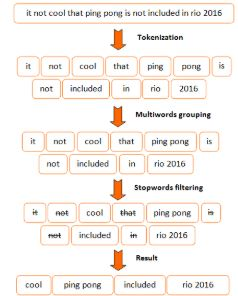
\includegraphics[scale=0.2]{figures/chapter-7-no-1-cahya.jpg}
\caption{Tokenizer - cahya}
\label{chapter-7-no-1-cahya}
\end{figure}
\par
\end{itemize}
\par
\par
\item Konsep Dasar K Fold Cross Validation Pada Dataset Komentar Youtube Pada Kode Listing Beserta Dengan Ilustrasi Gambar :
\item Jelaskan Apa Maksud Kode Program For Train Dan Test In Splits Dilengkapi Dengan Ilustrasi Gambar :
\item Apa Maksud Kode Program train\_content = d['CONTENT'].iloc[train\_idx] dan test\_content = d['CONTENT'].iloc[test\_idx] Dilengkapi Dengan Ilustrasi Gambar :
\item Apa Maksud Dari Fungsi Tokenizer = Tokenizer(num words=2000) Dan Tokenizer.fit on texts(train content), Dilengkapi Dengan Ilustrasi Gambar :
\item Apa Maksud Dari Fungsi d train inputs = tokenizer.texts to matrix(train content, mode=’tfidf ’) dan d test inputs = tokenizer.texts to matrix(test content, mode=’tfidf ’), Dilengkapi Dengan Ilustrasi Kode Dan Atau Gambar :
\item Apa Maksud Dari Fungsi d train inputs = d train inputs/np.amax(np.absolute(d\_train) :
\item Apa Maksud Dari Fungsi Di Listing ?? Dengan Parameter Tersebut. [caption=Compile model,label=lst:7.2] model.compile(loss=’categoricalcrossentropy0, optimizer =0 adamax0, metrics = [0accuracy0]) :
\item Apa itu Deep Learning :
\begin{itemize}
\item Penjelasan :
\par Deep learning merupakan sub bidang pembelajaran mesin yang berkaitan dengan algoritma.
\par
\end{itemize}
\item Apa itu Deep Neural Network Dan Apa Bedanya Dengan Deep Learning :
\begin{itemize}
\item Penjelasan Deep Neural Network : 
\par Deep neural network adalah jaringan syaraf dengan tingkat kompleksitas tertentu, jaringan syaraf dengan lebih dari dua lapisan.
\par
\item Perbedaan Deep Neural Network Dan Deep Learning :
\par Perbedaan antara deep neural network dan deep learning terletak pada kedalaman model. deep learning adalah frasa yang digunakan untuk jaringan saraf yang kompleks. Kompleksitas ini disebabkan oleh pola yang rumit tentang bagaimana informasi dapat mengalir di seluruh model.
\par
\par
\end{itemize}
\item Bagaimana Perhitungan Algoritma Dengan Ukuran Stride (NPM mod3+1)x(NPM mod3+1) Yang  Terdapat Pada Max Pooling :
\end{enumerate}


\subsection{Praktek}


\subsection{Penanganan Error}
